\documentclass[11pt,reqno]{amsart}

\usepackage[T1]{fontenc}
\usepackage[utf8]{inputenc}
\usepackage{lmodern}
\usepackage{amsmath,amssymb,amsthm,mathtools}
\usepackage{microtype}
\usepackage{booktabs}
\usepackage{enumitem}
\usepackage{tikz}
\usetikzlibrary{arrows.meta,positioning,fit}
\usepackage[colorlinks=true,linkcolor=blue,citecolor=blue,urlcolor=blue]{hyperref}
\usepackage[nameinlink,capitalise]{cleveref}

\newtheorem{theorem}{Theorem}[section]
\newtheorem{proposition}[theorem]{Proposition}
\newtheorem{lemma}[theorem]{Lemma}
\newtheorem{corollary}[theorem]{Corollary}
\newtheorem{remark}[theorem]{Remark}
\newtheorem{definition}[theorem]{Definition}

\newcommand{\C}{\mathbb C}
\newcommand{\N}{\mathbb N}
\newcommand{\Z}{\mathbb Z}
\newcommand{\cC}{\mathcal C}
\newcommand{\one}{\mathbf 1}
\newcommand{\Span}{\operatorname{span}}
\newcommand{\supp}{\operatorname{supp}}
\newcommand{\col}{\operatorname{col}}
\newcommand{\Jac}{\operatorname{J}}

\title[Fixed-parameter failure of subtree shuffling]
{An Explicit Fixed-Parameter Obstruction to Subtree Shuffling}

\author{Angus Muffatti}
\date{23 July 2026}

\subjclass[2020]{Primary 05C05, 14R15; Secondary 05A15, 13F25}
\keywords{Jacobian conjecture, Catalan trees, shuffle classes, Keller maps,
formal inversion, Lagrange inversion, nilpotent Jacobian}

\begin{document}

\begin{abstract}
Bisi, Dyszewski, Gantert, Johnston, Prochno, and Schmid conjectured that,
for fixed integers $d\geq2$ and $p\geq1$, the constant function on the set
of sufficiently large planar $d$-ary Catalan trees lies in the span of the
indicators of length-$p$ subtree-shuffle classes.

We give an explicit fixed-parameter obstruction.  For $d=7$, $p=15$, and
every $m\geq1$, the constant function on the $7$-Catalan trees with $3m$
internal vertices does not lie in the span of the length-$15$ shuffle
indicators.  If $M_{7,15,3m}$ is the tree-by-shuffle-class incidence matrix,
we construct an integer vector $w_m$ satisfying
\[
 M_{7,15,3m}^{\mathsf T}w_m=0,
 \qquad
 \one^{\mathsf T}w_m
 =(7!)^{3m}(-1)^m2^m\binom{3m+1}{m}\neq0.
\]

The construction starts from a three-dimensional noninjective Keller map.
A weighted Horner suspension produces a noninjective map
$\Phi=I-H:\C^{15}\to\C^{15}$ for which $H$ is homogeneous of degree seven
and $(JH)^{15}=0$.  An inverse-slice identity and Lagrange inversion give
infinitely many nonzero coefficients of the formal inverse of $\Phi$.
The shuffle lemma and tree-inverse formula then turn those coefficients
into the separating vectors above.

The same fixed pair disproves the corresponding shuffle-chain conjecture
and the all-degree extension of Singer's full-span conjecture.  The
separator vanishes on every $15$-perfect tree, so the exact obstruction is
supported on the exponentially rare exceptional family; this is compatible
with the previously proved asymptotic approximation theorem.
\end{abstract}

\maketitle

\section{Introduction}

Let $\cC_k^{(d)}$ be the set of rooted planar full $d$-ary trees with $k$
internal vertices.  Given an ancestral path of length $p$, one may rearrange
the $(d-1)p$ rooted subtrees attached to the siblings along that path.  The
set of distinct trees obtainable in this way is a length-$p$ shuffle class.
Bisi et al.\ introduced the following conjecture \cite[Conjecture~1.3]{BisiEtAl}.

\medskip
\noindent
\textbf{Subtree-shuffling conjecture.}
For every $d\geq2$ and $p\geq1$, there is $k_0(d,p)$ such that, for every
$k\geq k_0(d,p)$,
\[
 \one\in
 \Span\{\one_S:S\text{ is a length-$p$ shuffle class in }\cC_k^{(d)}\}.
\]
\medskip

The conjecture was designed as an unlabelled-tree route toward the Jacobian
conjecture.  Its origin lies in Singer's Catalan-tree approach
\cite{Singer2001,Singer2011}.  The subtree-shuffling preprint was posted on
19 January 2023 and appeared in final journal form on 22 January 2026.
The fixed certificate below is dated 23 July 2026, 1,281 days after the
preprint and 182 days after journal publication.

\begin{figure}[ht]
\centering
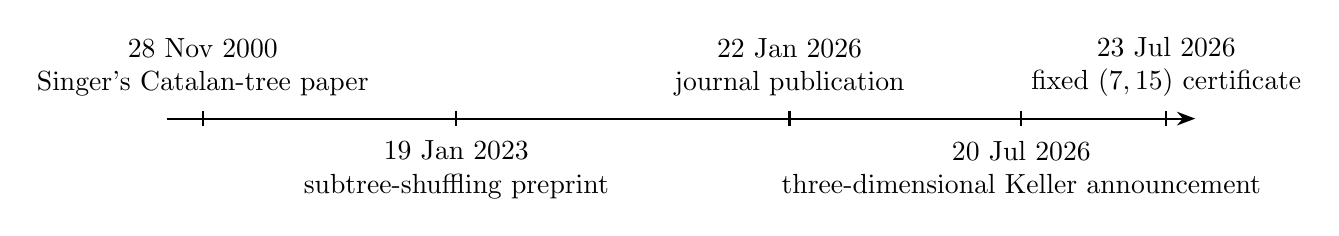
\begin{tikzpicture}[x=.92cm,y=1cm,>=Stealth]
  \draw[thick,->] (0,0)--(14.2,0);
  \foreach \x in {0.5,4.0,8.6,11.8,13.8} {\draw[thick] (\x,.10)--(\x,-.10);}
  \node[align=center,above] at (.5,.16) {28 Nov 2000\\Singer's Catalan-tree paper};
  \node[align=center,below] at (4,-.16) {19 Jan 2023\\subtree-shuffling preprint};
  \node[align=center,above] at (8.6,.16) {22 Jan 2026\\journal publication};
  \node[align=center,below] at (11.8,-.16) {20 Jul 2026\\three-dimensional Keller announcement};
  \node[align=center,above] at (13.8,.16) {23 Jul 2026\\fixed $(7,15)$ certificate};
\end{tikzpicture}
\caption{The combinatorial line of development.  The present result does
not decide Singer's original binary-tree conjecture; it refutes the later
all-degree extension at $d=7$.}
\label{fig:timeline}
\end{figure}

Our main result is the following fixed-parameter negation.

\begin{theorem}\label{thm:main}
For every integer $m\geq1$,
\[
 \one\notin
 \Span\{\one_S:S\text{ is a length-$15$ shuffle class in }
 \cC_{3m}^{(7)}\}.
\]
Consequently, the subtree-shuffling conjecture is false for the fixed pair
$(d,p)=(7,15)$.
\end{theorem}

The proof supplies a dual certificate.  Let $M_{d,p,k}$ denote the matrix
whose rows are indexed by $T\in\cC_k^{(d)}$, whose columns are indexed by the
distinct length-$p$ shuffle classes, and whose entries are
\[
 (M_{d,p,k})_{T,S}=\one_{\{T\in S\}}.
\]

\begin{theorem}\label{thm:certificate}
For every $m\geq1$, there exists an integer vector
$w_m\in\Z^{\cC_{3m}^{(7)}}$ such that
\[
 M_{7,15,3m}^{\mathsf T}w_m=0
\]
and
\[
 \one^{\mathsf T}w_m
 =(7!)^{3m}(-1)^m2^m\binom{3m+1}{m}\neq0.
\]
\end{theorem}

\begin{figure}[ht]
\centering
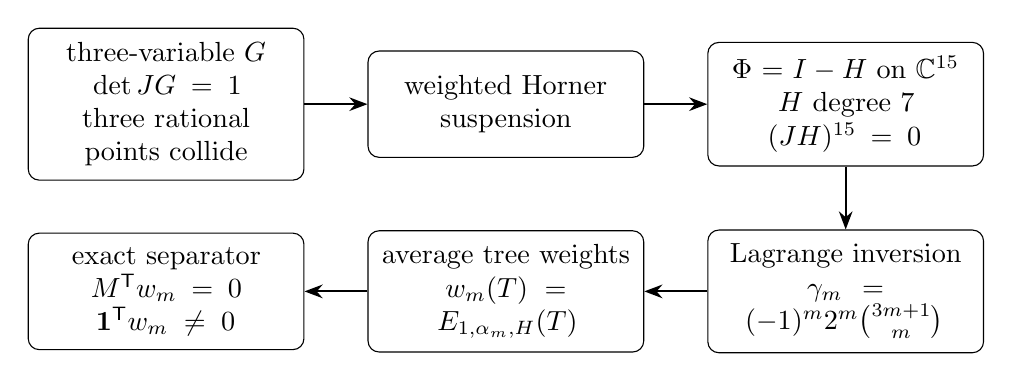
\begin{tikzpicture}[
 node distance=8mm and 8mm,
 box/.style={draw,rounded corners,align=center,text width=3.15cm,
              minimum height=1.35cm,inner sep=5pt},
 arrow/.style={-{Stealth[length=2.3mm]},thick}
]
\node[box] (g) {three-variable $G$\\$\det JG=1$\\three rational points collide};
\node[box,right=of g] (horner) {weighted Horner\\suspension};
\node[box,right=of horner] (phi) {$\Phi=I-H$ on $\C^{15}$\\$H$ degree $7$\\$(JH)^{15}=0$};
\node[box,below=of phi] (lagrange) {Lagrange inversion\\$\gamma_m=(-1)^m2^m\binom{3m+1}{m}$};
\node[box,left=of lagrange] (weight) {average tree weights\\$w_m(T)=E_{1,\alpha_m,H}(T)$};
\node[box,left=of weight] (sep) {exact separator\\$M^{\mathsf T}w_m=0$\\$\one^{\mathsf T}w_m\neq0$};
\draw[arrow] (g)--(horner);
\draw[arrow] (horner)--(phi);
\draw[arrow] (phi)--(lagrange);
\draw[arrow] (lagrange)--(weight);
\draw[arrow] (weight)--(sep);
\end{tikzpicture}
\caption{The proof pipeline.}
\label{fig:pipeline}
\end{figure}

The crucial point is explicitness.  A noninjective Keller map makes the
universal subtree-shuffling conjecture logically untenable once combined
with the implication of Bisi et al.; the present argument isolates a single
fixed degree, a single fixed path length, infinitely many tree sizes, and an
exact left-kernel vector.

\section{Shuffle duality and the separation principle}

We recall the two ingredients from \cite{BisiEtAl} that translate formal
inversion into unlabelled-tree linear algebra.

Let $H=(H_1,\ldots,H_n)$ be homogeneous of degree $d$, written in factorial
normalization as
\[
 H_i(X)=\sum_{|\beta|=d} H_{i,\beta}\frac{X^\beta}{\beta!}.
\]
For $T\in\cC_k^{(d)}$, a root type $i\in[n]$, and a leaf-type
multi-index $\alpha\in\Z_{\geq0}^n$ of size $(d-1)k+1$, let
$E_{i,\alpha,H}(T)$ be the sum of the $H$-weights of all type-labellings of
$T$ having root type $i$ and leaf multiplicities $\alpha$.

The shuffle lemma \cite[Lemma~3.3]{BisiEtAl} states that if
$(JH)^p=0$, with $1\leq p\leq n$, then
\begin{equation}\label{eq:shuffle-orthogonality}
 \sum_{T\in S}E_{i,\alpha,H}(T)=0
\end{equation}
for every length-$p$ shuffle class $S$.

If $F=I-H$, then its formal inverse has an expansion
\[
 (F^{-1})_i(X)=X_i+
 \sum_{k\geq1}\ \sum_{|\alpha|=(d-1)k+1}g_{i,\alpha}X^\alpha,
\]
and the tree-inverse formula is
\begin{equation}\label{eq:tree-inverse}
 g_{i,\alpha}
 =\frac{1}{(d!)^k}
 \sum_{T\in\cC_k^{(d)}}E_{i,\alpha,H}(T).
\end{equation}

\begin{proposition}[Separation principle]\label{prop:separation}
Suppose $H$ is homogeneous of degree $d$, $(JH)^p=0$, and
$g_{i,\alpha}\neq0$ for some $|\alpha|=(d-1)k+1$.  Define
\[
 w(T)=E_{i,\alpha,H}(T),\qquad T\in\cC_k^{(d)}.
\]
Then
\[
 M_{d,p,k}^{\mathsf T}w=0,
 \qquad
 \one^{\mathsf T}w=(d!)^k g_{i,\alpha}\neq0.
\]
In particular, $\one\notin\col M_{d,p,k}$.
\end{proposition}

\begin{proof}
Equation \eqref{eq:shuffle-orthogonality} is precisely
$M_{d,p,k}^{\mathsf T}w=0$.  Equation \eqref{eq:tree-inverse} gives the
total sum.  If $\one=M\lambda$, then
\[
 \one^{\mathsf T}w=\lambda^{\mathsf T}M^{\mathsf T}w=0,
\]
a contradiction.
\end{proof}

\section{A normalized three-dimensional Keller map}

Consider $G=(A,B,C):\C^3\to\C^3$ given by
\begin{align}
A={}&x-3x^2y-x^3z,\label{eq:A}\\
B={}&y+3xz+24xy^2+12x^2yz+36x^2y^3+12x^3y^2z,\label{eq:B}\\
C={}&z+8y^2+6xyz+28xy^3+12x^2y^2z+24x^2y^4+8x^3y^3z.
\label{eq:C}
\end{align}

This is the identity-linear determinant-one normalization of the
three-dimensional map discussed in 2026; a contemporaneous account of the
announcement appears in \cite{Long2026}.  The exact source and target
normalization is recorded in the reproducibility files.

\begin{proposition}\label{prop:G}
The map $G$ satisfies $\det JG=1$, and
\[
 G\left(0,0,-\frac18\right)
 =G\left(1,-\frac34,\frac{13}{4}\right)
 =G\left(-1,\frac34,\frac{13}{4}\right)
 =\left(0,0,-\frac18\right).
\]
\end{proposition}

\begin{proof}
The collisions follow by direct substitution.  For the determinant, put
\[
 u=1+2xy,
 \qquad
 r=\frac{x}{u}.
\]
On the dense open set $u\neq0$, direct simplification gives
\begin{equation}\label{eq:hidden}
 B=y+3rC,
 \qquad
 A=r-r^2B+2r^3C.
\end{equation}
The coordinate change $(x,y,z)\mapsto(r,y,C)$ has determinant
\[
 \frac{\partial r}{\partial x}\frac{\partial C}{\partial z}
 =\frac{1}{u^2}u^3=u.
\]
The change $(r,y,C)\mapsto(C,B,r)$ has determinant $-1$.  Holding $B,C$
fixed in the second identity of \eqref{eq:hidden} gives
\[
 \frac{\partial A}{\partial r}
 =1-2rB+6r^2C
 =1-2ry
 =\frac1u.
\]
Thus the determinant of the map to $(C,B,A)$ is $-1$.  Swapping the first
and third target coordinates gives $\det JG=1$ on $u\neq0$, hence
everywhere by polynomial continuation.
\end{proof}

\section{Weighted Horner suspension}

We next give the construction that turns a nonhomogeneous identity-linear
Keller map into a homogeneous Keller map while retaining a controlled
nilpotency index.

Let
\[
 G_i(X)=X_i+\sum_{j=2}^{d_i}K_{i,j}(X),
\]
where $K_{i,j}$ is homogeneous of degree $j$.  Introduce auxiliary variables
$Y_{i,3},\ldots,Y_{i,d_i}$ and let
\[
 M=n+\sum_{i=1}^n(d_i-2).
\]
Define $N:\C^M\to\C^M$ by
\begin{align}
 N_{X_i}&=K_{i,2}(X)+Y_{i,3},\label{eq:Nx}\\
 N_{Y_{i,j}}&=-K_{i,j}(X)-Y_{i,j+1},
 &&3\leq j<d_i,\label{eq:Ny}\\
 N_{Y_{i,d_i}}&=-K_{i,d_i}(X).\label{eq:Nlast}
\end{align}

\begin{theorem}[Weighted Horner suspension]\label{thm:horner}
Assume $\det JG=1$.  Then
\[
 (JN)^M=0.
\]
Let $d=\max_i d_i$, add one variable $h$, and define
\[
 \mathcal H(Z,h)=\left(h^dN\left(\frac Zh\right),0\right).
\]
Then $\mathcal H$ is homogeneous of degree $d$ and
\[
 (J\mathcal H)^{M+1}=0.
\]
Consequently, $\Phi=I+\mathcal H$ has Jacobian determinant one.

Moreover, every collision of $G$ lifts to a collision of $\Phi$ on the
hyperplane $h=1$.
\end{theorem}

\begin{proof}
For an indeterminate $s$, put $U_s=I+sN$.  Thus
\begin{align*}
 X_i'&=X_i+sK_{i,2}(X)+sY_{i,3},\\
 Y_{i,j}'&=Y_{i,j}-sK_{i,j}(X)-sY_{i,j+1},\\
 Y_{i,d_i}'&=Y_{i,d_i}-sK_{i,d_i}(X).
\end{align*}
The weighted Horner identity is
\begin{equation}\label{eq:telescoping}
 X_i'-\sum_{j=3}^{d_i}s^{j-2}Y_{i,j}'
 =X_i+\sum_{j=2}^{d_i}s^{j-1}K_{i,j}(X)
 =s^{-1}G_i(sX).
\end{equation}
The operation on the left is a target shear of determinant one.  After this
shear, the original-coordinate outputs depend only on $X$, while the
auxiliary-output Jacobian with respect to the auxiliary variables is unit
triangular.  Hence
\[
 \det(I+sJN)
 =\det J\bigl(s^{-1}G(sX)\bigr)
 =\det JG(sX)
 =1.
\]
It follows that the characteristic polynomial of $JN$ is $\lambda^M$.
Cayley--Hamilton gives $(JN)^M=0$.

The expression $h^dN(Z/h)$ is homogeneous of degree $d$.  On $h\neq0$,
its Jacobian has block form
\[
 J\mathcal H=
 \begin{pmatrix}
 h^{d-1}JN(Z/h)& *\\
 0&0
 \end{pmatrix}.
\]
The $(M+1)$st power vanishes because $(JN)^M=0$.  Since the entries are
polynomials, the identity extends to $h=0$.

For the collision statement, at $h=1$ set
\[
 Y_{i,j}=\sum_{\ell=j}^{d_i}K_{i,\ell}(q).
\]
Then all auxiliary outputs telescope to zero, and the $i$th original output
is $G_i(q)$.  Equal $G$-images therefore yield equal $\Phi$-images.
\end{proof}

The construction also controls a slice of the formal inverse.

\begin{proposition}[Inverse slice]\label{prop:inverse-slice}
Let $\pi_X$ project onto the original $n$ coordinates.  If all auxiliary
target coordinates vanish, then
\[
 \pi_X\Phi^{-1}(A,0,h)
 =h^{-(d-2)}G^{-1}\bigl(h^{d-2}A\bigr)
\]
as an identity of formal power series.
\end{proposition}

\begin{proof}
Write $Z=hz$ and $s=h^{d-1}$.  Then
\[
 \Phi(Z,h)=\bigl(hU_s(z),h\bigr).
\]
When the auxiliary target coordinates are zero, the target shear in
\eqref{eq:telescoping} leaves the original target coordinates unchanged.
Thus
\[
 s^{-1}G(sx)=\frac Ah,
 \qquad
 G(sx)=h^{d-2}A.
\]
Therefore $sx=G^{-1}(h^{d-2}A)$, while the original coordinates of $Z$ are
$hx$.  Since $h/s=h^{-(d-2)}$, the formula follows.
\end{proof}

\section{The explicit homogeneous map in fifteen variables}

For \eqref{eq:A}--\eqref{eq:C}, the component degrees are
\[
 (d_1,d_2,d_3)=(4,6,7),
\]
so $M=14$ before homogenization and $M+1=15$ afterwards.  Use coordinates
\[
 x,y,z,a_3,a_4,b_3,b_4,b_5,b_6,c_3,c_4,c_5,c_6,c_7,h.
\]
The suspended map is
\begin{align*}
\Phi_x={}&x+a_3h^6,\\
\Phi_y={}&y+3xzh^5+b_3h^6,\\
\Phi_z={}&z+8y^2h^5+c_3h^6,\\
\Phi_{a_3}={}&a_3+3x^2yh^4-a_4h^6,\\
\Phi_{a_4}={}&a_4+x^3zh^3,\\
\Phi_{b_3}={}&b_3-24xy^2h^4-b_4h^6,\\
\Phi_{b_4}={}&b_4-12x^2yzh^3-b_5h^6,\\
\Phi_{b_5}={}&b_5-36x^2y^3h^2-b_6h^6,\\
\Phi_{b_6}={}&b_6-12x^3y^2zh,\\
\Phi_{c_3}={}&c_3-6xyzh^4-c_4h^6,\\
\Phi_{c_4}={}&c_4-28xy^3h^3-c_5h^6,\\
\Phi_{c_5}={}&c_5-12x^2y^2zh^2-c_6h^6,\\
\Phi_{c_6}={}&c_6-24x^2y^4h-c_7h^6,\\
\Phi_{c_7}={}&c_7-8x^3y^3z,\\
\Phi_h={}&h.
\end{align*}

\begin{corollary}\label{cor:explicit-map}
Write $\Phi=I-H$.  Then $H$ is homogeneous of degree seven,
\[
 (JH)^{15}=0,
 \qquad
 \det J\Phi=1,
\]
and $\Phi$ is not injective.
\end{corollary}

\begin{proof}
Homogeneity and nilpotency follow from \cref{thm:horner}.  Noninjectivity
follows by lifting the three points in \cref{prop:G}.  For completeness,
put
\[
 Q_0=\left(0,0,-\frac18,0,0,0,0,0,0,0,0,0,0,0,1\right)
\]
and, for $\varepsilon\in\{1,-1\}$,
\[
\begin{split}
 Q_\varepsilon=\bigg(&
 \varepsilon,-\frac{3\varepsilon}{4},\frac{13}{4},
 -\varepsilon,-\frac{13\varepsilon}{4},
 -9\varepsilon,-\frac{45\varepsilon}{2},
 \frac{27\varepsilon}{4},\frac{351\varepsilon}{16},\\
 &-\frac{63}{8},\frac{27}{4},\frac{297}{16},
 -\frac{27}{8},-\frac{351}{32},1\bigg).
\end{split}
\]
Direct substitution gives
\[
 \Phi(Q_0)=\Phi(Q_1)=\Phi(Q_{-1})=Q_0.
\]
\end{proof}

\section{A nonzero inverse coefficient}

Let $(A,B,C)=G(x,y,z)$ and put $r=x/(1+2xy)$.  On the target plane $B=0$,
\eqref{eq:hidden} becomes
\begin{equation}\label{eq:cubic-slice}
 A=r+2Cr^3,
 \qquad
 y=-3Cr.
\end{equation}
Moreover,
\[
 x=\frac{r}{1+6Cr^2}
 =r\frac{\partial r}{\partial A}
 =\frac12\frac{\partial(r^2)}{\partial A}.
\]

\begin{proposition}\label{prop:gamma}
For every $m\geq0$,
\[
 [A^{2m+1}C^m](G^{-1})_1
 =\gamma_m
 :=(-1)^m2^m\binom{3m+1}{m}.
\]
In particular, $\gamma_m\neq0$.
\end{proposition}

\begin{proof}
Equation \eqref{eq:cubic-slice} is equivalent to
\[
 r=A(1+2Cr^2)^{-1}.
\]
The Lagrange--B\"urmann formula gives
\[
 [A^{2m+2}]r^2
 =\frac{2}{2m+2}[t^{2m}](1+2Ct^2)^{-(2m+2)}
 =\frac{(-1)^m2^m}{m+1}\binom{3m+1}{m}C^m.
\]
Applying $\frac12\partial/\partial A$ gives the result.
\end{proof}

By \cref{prop:inverse-slice}, with $d=7$,
\[
 (\Phi^{-1})_1(A,0,h)=h^{-5}(G^{-1})_1(h^5A).
\]
Consequently,
\begin{equation}\label{eq:phi-coefficient}
 [A^{2m+1}C^mh^{15m}](\Phi^{-1})_1=\gamma_m.
\end{equation}
The total degree is
\[
 (2m+1)+m+15m=18m+1=6(3m)+1,
\]
which is the leaf count of a $7$-ary Catalan tree with $3m$ internal
vertices.

\section{Proof of the fixed-parameter obstruction}

Set
\[
 \alpha_m=(2m+1,0,m,\underbrace{0,\ldots,0}_{11\text{ auxiliary types}},15m)
 \in\Z_{\geq0}^{15}.
\]
Then $|\alpha_m|=18m+1$.  For $T\in\cC_{3m}^{(7)}$, define
\begin{equation}\label{eq:def-w}
 w_m(T)=E_{1,\alpha_m,H}(T),
\end{equation}
where $\Phi=I-H$ is the explicit map of the previous section.

\begin{proof}[Proof of \cref{thm:certificate}]
By \cref{cor:explicit-map}, $(JH)^{15}=0$.  The shuffle lemma with
$n=p=15$ gives
\[
 \sum_{T\in S}w_m(T)=0
\]
for every length-$15$ shuffle class $S$, hence
\[
 M_{7,15,3m}^{\mathsf T}w_m=0.
\]

By the tree-inverse formula and \eqref{eq:phi-coefficient},
\begin{align*}
 \one^{\mathsf T}w_m
 &=\sum_{T\in\cC_{3m}^{(7)}}E_{1,\alpha_m,H}(T)\\
 &=(7!)^{3m}[A^{2m+1}C^mh^{15m}](\Phi^{-1})_1\\
 &=(7!)^{3m}(-1)^m2^m\binom{3m+1}{m}.
\end{align*}
This is nonzero.

The ordinary coefficients of $H$ are integers.  In factorial normalization,
$H_{i,\beta}$ is the ordinary coefficient multiplied by $\beta!$, and is
therefore an integer.  Formula \eqref{eq:def-w} is a finite sum of products
of such integers, so $w_m$ is integer-valued.
\end{proof}

\begin{proof}[Proof of \cref{thm:main}]
Apply \cref{prop:separation,thm:certificate}.
\end{proof}

The result is not merely caused by small trees having no path of length
$15$.

\begin{proposition}[Fully covered regime]\label{prop:covered}
Every $7$-ary Catalan tree with
\[
 k\geq113037178809
\]
has a path of length $15$.  The first such $k$ is divisible by three, and
\cref{thm:main} applies there.
\end{proposition}

\begin{proof}
If a full $7$-ary tree has no path of length $15$, its internal vertices can
occur only at depths $0,\ldots,13$.  Hence it has at most
\[
 1+7+\cdots+7^{13}=\frac{7^{14}-1}{6}=113037178808
\]
internal vertices.  The next integer is
\[
 113037178809=3\cdot37679059603.
\]
\end{proof}

\section{Exact failure and asymptotic approximation}

A $15$-perfect tree contains a length-$15$ path whose off-path sibling
subtrees are all leaves.  Such a path defines a singleton shuffle class.
Applying the shuffle identity to that singleton gives
\[
 w_m(T)=0
\]
for every $15$-perfect tree.  Thus
\[
 \supp w_m\subseteq
 \{T\in\cC_{3m}^{(7)}:T\text{ is not $15$-perfect}\}.
\]

Bisi et al.\ prove that, for fixed $d,p$, the proportion of non-$p$-perfect
trees decays exponentially in $k$ \cite[Theorem~1.7]{BisiEtAl}.  The exact
separator is therefore supported on an exponentially rare exceptional
family.  This explains how exact spanning can fail while their unconditional
$\ell^1$ and $\ell^\infty$ approximation theorem remains valid.

\begin{figure}[ht]
\centering
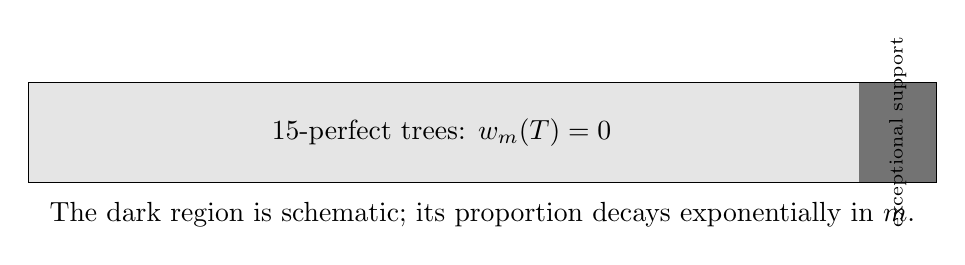
\begin{tikzpicture}[x=.095\textwidth,y=1cm]
  \draw[thick] (0,0) rectangle (10,1.25);
  \fill[black!10] (0,0) rectangle (9.15,1.25);
  \fill[black!55] (9.15,0) rectangle (10,1.25);
  \node at (4.55,.63) {$15$-perfect trees: $w_m(T)=0$};
  \node[rotate=90] at (9.58,.63) {\scriptsize exceptional support};
  \node[below,align=center] at (5,-.13)
  {The dark region is schematic; its proportion decays exponentially in $m$.};
\end{tikzpicture}
\caption{The exact obstruction lives only on the rare non-perfect trees.}
\label{fig:rarity}
\end{figure}

\section{Consequences and scope}

\begin{corollary}\label{cor:chain}
For $d=7$ and $p=15$, the shuffle-chain conjecture of Bisi et al.\ fails for
infinitely many tree sizes $k$, namely every $k=3m$.
\end{corollary}

\begin{proof}
A length-$p$ shuffle chain with the uniform stationary distribution produces
a nonnegative representation of the constant function by length-$p$
shuffle-class indicators \cite[Theorem~1.6 and its proof]{BisiEtAl}.  Such a
representation is impossible by \cref{thm:main}.
\end{proof}

\begin{corollary}\label{cor:singer}
The all-degree extension of Singer's full-span conjecture fails for
$d=7$, $p=15$, and every $k=3m$.
\end{corollary}

\begin{proof}
Full spanning would in particular span the constant function.
\end{proof}

\begin{remark}
\Cref{cor:singer} does not decide Singer's original binary-tree conjecture.
It refutes the later formulation in which $d$ is allowed to be arbitrary.
\end{remark}

The construction does not establish minimality.  Natural open problems are
to determine the least failing $d$, the least failing $p$ for that $d$, the
least possible homogeneous degree and dimension, and a direct unlabelled
combinatorial description of the support and signs of $w_m$.

\section{Reproducibility and verification}

The accompanying repository contains:
\begin{enumerate}[label=(\roman*)]
\item exact SymPy checks of the Jacobian determinants and collisions;
\item a generic implementation of the weighted Horner suspension;
\item symbolic checks of the telescoping identities and unit-triangular
      auxiliary block;
\item exact integer matrix-power regression checks at several
      specializations;
\item fixed-point formal-series checks of the Lagrange coefficient;
\item tests enforcing the fixed claim $(d,p)=(7,15)$;
\item a continuous-integration workflow that runs the checks and compiles
      this manuscript.
\end{enumerate}

The matrix-power specializations are regression tests, not substitutes for
the symbolic proof.  The proof of nilpotency is the identity
$\det(I+sJN)=1$ together with Cayley--Hamilton and the homogenized block
argument in \cref{thm:horner}.

\section*{Provenance and responsibility}

The starting three-dimensional polynomial map was supplied in the research
discussion leading to this manuscript.  The normalization, weighted Horner
suspension, inverse-slice identity, coefficient extraction, and fixed
shuffle certificate are documented here and in the repository history.
Before submission, the human contributors must settle authorship,
acknowledgements, and any journal-required disclosure of AI-assisted
research and drafting.  The named authors bear responsibility for every
mathematical and historical claim.

\begin{thebibliography}{99}

\bibitem{BCW}
H.~Bass, E.~H. Connell, and D.~Wright,
\emph{The Jacobian conjecture: reduction of degree and formal expansion of
the inverse},
Bull. Amer. Math. Soc. (N.S.) \textbf{7} (1982), 287--330.

\bibitem{BisiEtAl}
E.~Bisi, P.~Dyszewski, N.~Gantert, S.~G.~G. Johnston, J.~Prochno,
and D.~Schmid,
\emph{Random planar trees and the Jacobian conjecture},
J. London Math. Soc. \textbf{113} (2026), e70416.
\url{https://doi.org/10.1112/jlms.70416}.

\bibitem{JohnstonProchno}
S.~G.~G. Johnston and J.~Prochno,
\emph{Fa\`a di Bruno's formula and inversion of power series},
Adv. Math. \textbf{395} (2022), 108080.

\bibitem{Keller}
O.-H. Keller,
\emph{Ganze Cremona-Transformationen},
Monatsh. Math. Phys. \textbf{47} (1939), 299--306.

\bibitem{Long2026}
C.~D. Long,
\emph{Small counterexamples to the Gaussian Moments Conjecture},
arXiv:2607.18186, 2026.

\bibitem{Singer2001}
D.~Singer,
\emph{On Catalan trees and the Jacobian conjecture},
Electron. J. Combin. \textbf{8} (2001), Research Paper R2.

\bibitem{Singer2011}
D.~Singer,
\emph{Toward a combinatorial proof of the Jacobian conjecture!},
Electron. J. Combin. \textbf{18} (2011), Paper P27.

\bibitem{vanDenEssen}
A.~van den Essen,
\emph{Polynomial Automorphisms and the Jacobian Conjecture},
Progress in Mathematics 190, Birkh\"auser, 2000.

\end{thebibliography}

\end{document}
